\documentclass{article}
\iffalse
This file is protected by Copyright. Please refer to the COPYRIGHT file
distributed with this source distribution.

This file is part of OpenCPI <http://www.opencpi.org>

OpenCPI is free software: you can redistribute it and/or modify it under the
terms of the GNU Lesser General Public License as published by the Free Software
Foundation, either version 3 of the License, or (at your option) any later
version.

OpenCPI is distributed in the hope that it will be useful, but WITHOUT ANY
WARRANTY; without even the implied warranty of MERCHANTABILITY or FITNESS FOR A
PARTICULAR PURPOSE. See the GNU Lesser General Public License for more details.

You should have received a copy of the GNU Lesser General Public License along
with this program. If not, see <http://www.gnu.org/licenses/>.
\fi

\author{} % Force author to be blank
%----------------------------------------------------------------------------------------
% Paper size, orientation and margins
%----------------------------------------------------------------------------------------
\usepackage{geometry}
\geometry{
	letterpaper,			% paper type
	portrait,				% text direction
	left=.75in,				% left margin
	top=.75in,				% top margin
	right=.75in,			% right margin
	bottom=.75in			% bottom margin
 }
%----------------------------------------------------------------------------------------
% Header/Footer
%----------------------------------------------------------------------------------------
\usepackage{fancyhdr} \pagestyle{fancy} % required for fancy headers
\renewcommand{\headrulewidth}{0.5pt}
\renewcommand{\footrulewidth}{0.5pt}
\rhead{\small{ANGRYVIPER Team}}
%----------------------------------------------------------------------------------------
% Appendix packages
%----------------------------------------------------------------------------------------
\usepackage[toc,page]{appendix}
%----------------------------------------------------------------------------------------
% Defined Commands & Renamed Commands
%----------------------------------------------------------------------------------------
\renewcommand{\contentsname}{Table of Contents}
\renewcommand{\listfigurename}{List of Figures}
\renewcommand{\listtablename}{List of Tables}
\newcommand{\todo}[1]{\textcolor{red}{TODO: #1}\PackageWarning{TODO:}{#1}} % To do notes
\newcommand{\code}[1]{\texttt{#1}} % For inline code snippet or command line
%----------------------------------------------------------------------------------------
% Various pacakges
%----------------------------------------------------------------------------------------
\usepackage{hyperref} % for linking urls and lists
\usepackage{graphicx} % for including pictures by file
\usepackage{listings} % for coding language styles
\usepackage{rotating} % for sideways table
\usepackage{pifont}   % for sideways table
\usepackage{pdflscape} % for landscape view
%----------------------------------------------------------------------------------------
% Table packages
%----------------------------------------------------------------------------------------
\usepackage{tabularx} % c=center,l=left,r=right,X=fill
\usepackage{float}
\floatstyle{plaintop}
\usepackage[tableposition=top]{caption}
\newcolumntype{P}[1]{>{\centering\arraybackslash}p{#1}}
\newcolumntype{M}[1]{>{\centering\arraybackslash}m{#1}}
%----------------------------------------------------------------------------------------
% Block Diagram / FSM Drawings
%----------------------------------------------------------------------------------------
\usepackage{tikz}
\usetikzlibrary{shapes,arrows,fit,positioning}
\usetikzlibrary{automata} % used for the fsm
%----------------------------------------------------------------------------------------
% Colors Used
%----------------------------------------------------------------------------------------
\usepackage{colortbl}
\definecolor{blue}{rgb}{.7,.8,.9}
\definecolor{ceruleanblue}{rgb}{0.16, 0.32, 0.75}
\definecolor{drkgreen}{rgb}{0,0.6,0}
\definecolor{deepmagenta}{rgb}{0.8, 0.0, 0.8}
\definecolor{cyan}{rgb}{0.0,0.6,0.6}
\definecolor{maroon}{rgb}{0.5,0,0}
%----------------------------------------------------------------------------------------
% Update the docTitle and docVersion per document
%----------------------------------------------------------------------------------------
\def\docTitle{Component Data Sheet}
\def\docVersion{1.3}
%----------------------------------------------------------------------------------------
\date{Version \docVersion} % Force date to be blank and override date with version
\title{\docTitle}
\lhead{\small{\docTitle}}

\def\comp{lime\_tx\_proxy}
\edef\ecomp{lime_tx_proxy}
\def\Comp{Lime TX Proxy}
\graphicspath{ {figures/} }

\begin{document}

\section*{Summary - \Comp}
\begin{tabular}{|c|M{13.5cm}|}
	\hline
	\rowcolor{blue}
	                  &                \\
	\hline
	Name              & \comp          \\
	\hline
	Worker Type       & Proxy          \\
	\hline
	Version           & v\docVersion \\
	\hline
	Release Date      & February 2018 \\
	\hline
	Component Library & ocpi.assets.devices   \\
	\hline
	Workers           & \comp.rcc      \\
	\hline
	Tested Platforms  & xilinx13\_3, CentOS 7 (via alst4/Zipper), CentOS 6/7 (via ml605/Zipper for HPC and LPC FMC slots) \\
	\hline
	Slave Worker      & lime\_tx.hdl   \\
	\hline
\end{tabular}

\section*{Functionality}
This control proxy is designed to allow the user of the proxy to set more user friendly properties than the register map on the LMS6002D Transceiver.  Only the control of the TX portion of the LMS6002D Transceiver is encompassed in this worker.

\section*{Worker Implementation Details}
\subsection*{\comp.rcc}
% hardcoded figure 2 because I cant figure out how to refence a figure in another section
A diagram of the transmitter in the Lime Microsystems LMS6002D can be seen in figure 2. The FPGA provides complex samples to the LMS6002D on a 12 bit multiplexed bus, and analog IQ signals are generated by on chip DACs. These signals then pass through a low pass filters and a programmable gain amplifier. After the first amplifier stage, DC offset is inserted in the IQ path in order to cancel the LO leakage. The IQ signals are then mixed with a PLL output to produce a modulated RF signal. This RF signal is then split and amplified by two separate controllable gain amplifiers, only one of which can be active at any given time, limiting the device to a single transmit channel. After the second amplifier stage, the RF signal is routed to an output pin on the transceiver.\par\bigskip
\noindent The features described above are controllable via a SPI interface on the LMS6002D. This proxy is responsible for translating its properties (as described in the Lime datasheet) into the required SPI reads and writes and controlling the worker which performs the SPI transactions.
\newpage

\section*{Block Diagrams}
\subsection*{Top level}
\begin{figure}[ht]
	\centerline{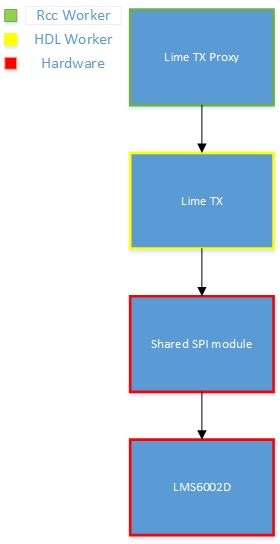
\includegraphics[scale=0.7]{lime_TX_toplevel}}
	\caption{Top Level Block Diagram}
	\label{fig:top}
\end{figure}
\vspace{25 mm}

\subsection*{Hardware}
\begin{figure}[ht]
	\centerline{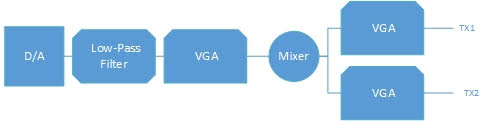
\includegraphics[scale=0.7]{lime_TX_HW}}
	\caption{Hardware Block Diagram}
	\label{fig:hw}
\end{figure}
\vspace{25 mm}

\section*{Source Dependencies}
\begin{itemize}
	\item assets/hdl/devices/lime\_tx\_proxy.rcc/lime\_tx\_proxy.cc
\end{itemize}

\begin{landscape}
	\section*{Component Spec Properties}
	\begin{scriptsize}
		\begin{tabular}{|p{3cm}|c|c|c|c|c|c|p{10cm}|}
			\hline
			\rowcolor{blue}
			Name                         & Type   & Sequence & Array      & Accessibility       & Valid & Default & Usage                                                                                                                                                                                                                       \\
			\rowcolor{blue}
			                             &        & Length   & Dimensions &                     & Range &         &                                                                                                                                                                                                                             \\
			\hline
			\verb+lpf_bw_hz+             & Float  & -        & -          & Writable, Readable  & -     & -       & The low pass filter that is used to filter out any noise on the received signal.                                                                                                                                            \\
			\hline
			\verb+post_lpf_gain_db+      & Short  & -        & -          & Writable, Readable  & -     & -       & The gain value for the VGA in after the low pass filter. The value is in dB and can only be set in multiples of 3.                                                                                                          \\
			\hline
			\verb+pre_mixer_dc_offset_i+ & UChar  & -        & -          & Writable, Readable  & -     & -       & The register value used to tune the DC offset of the transmitted signal to close to zero on the I path.                                                                                                                     \\
			\hline
			\verb+pre_mixer_dc_offset_q+ & UChar  & -        & -          & Writable, Readable  & -     & -       & The register value used to tune the DC offset of the transmitted signal to close to zero on the Q path.                                                                                                                     \\
			\hline
			\verb+center_freq_hz+        & Double & -        & -          & Writable, Readable  & -     & -       & The value of the tuned center frequency of the transmitter.                                                                                                                                                                 \\
			\hline
			\verb+output_gain_db+        & Short  & -        & -          & Writable, Readable  & -     & -       & The gain value for the VGA in after the mixer.                                                                                                                                                                              \\
			\hline
			\verb+noutputs+              & UChar  & -        & -          & Readable, Parameter & 1-2   & 1       & The number of hardware outputs that are available to this TX interface.                                                                                                                                                     \\
			\hline
			\verb+output_select+         & UChar  & -        & -          & Writable, Readable  & -     & -       & This is the hardware selection of which output to pass the mixer output of the mixer to. The two outputs are identical, but on a given platform, there could be different analog hardware connected outside of the LMS6002D. \\
			\hline
		\end{tabular}
	\end{scriptsize}

	\section*{Worker Properties}
	\subsection*{\comp.rcc}
	\begin{scriptsize}
		\begin{tabular}{|p{2cm}|p{3cm}|c|c|c|c|p{2.5cm}|c|p{7cm}|}
			\hline
			\rowcolor{blue}
			Type         & Name                         & Type & Sequence & Array      & Accessibility/ & Valid Range                                                                                                    & Default & Usage                                                                                                                                                                                                                       \\
			\rowcolor{blue}
			             &                              &      & Length   & Dimensions & Advanced       &                                                                                                                &         &                                                                                                                                                                                                                             \\
			\hline
			SpecProperty & \verb+lpf_bw_hz+             & -    & -        & -          & WriteSync      & 14e6, 10e6, 7e6, 6e6, 5e6, 4.375e6, 3.5e6, 3e6, 2.75e6, 2.5e6, 1.92e6, 1.5e6, 1.375e6, 1.25e6, 0.875e6, 0.75e6 & -       & The low pass filter that is used to filter out any noise on the received signal.                                                                                                                                            \\
			\hline
			SpecProperty & \verb+post_lpf_gain_db+      & -    & -        & -          & WriteSync      & -4 to -35                                                                                                      & -       & The gain value for the VGA in after the low pass filter. The value is in dB and can only be set in multiples of 3.                                                                                                          \\
			\hline
			SpecProperty & \verb+pre_mixer_dc_offset_i+ & -    & -        & -          & WriteSync      & 0x00-0x80                                                                                                      & -       & The register value used to tune the DC offset of the transmitted signal to close to zero on the I path.                                                                                                                     \\
			\hline
			SpecProperty & \verb+pre_mixer_dc_offset_q+ & -    & -        & -          & WriteSync      & 0x00-0x80                                                                                                      & -       & The register value used to tune the DC offset of the transmitted signal to close to zero on the Q path.                                                                                                                     \\
			\hline
			SpecProperty & \verb+center_freq_hz+        & -    & -        & -          & WriteSync      & 232,500 - 3,720,000                                                                                            & -       & The value of the tuned center frequency of the transmitter.                                                                                                                                                                 \\
			\hline
			SpecProperty & \verb+output_gain_db+        & -    & -        & -          & WriteSync      & 0-25                                                                                                           & -       & The gain value for the VGA in after the mixer.                                                                                                                                                                              \\
			\hline
			SpecProperty & \verb+noutputs+              & -    & -        & -          & -              & 2                                                                                                              & 2       & The number of hardware outputs that are available to this TX interface.                                                                                                                                                     \\
			\hline
			SpecProperty & \verb+output_select+         & -    & -        & -          & WriteSync      & 1-2                                                                                                            & -       & This is the hardware selection of which output to pass the mixer output of the mixer to. The two outputs are identical, but on a given platform, there could be different analog hardware connected outside of the LMS6002D. \\
			\hline
		\end{tabular}
	\end{scriptsize}
\end{landscape}

\section*{Performance and Resource Utilization}
\subsubsection*{\comp.rcc}
\begin{scriptsize}
	\begin{tabular}{|c|c|c|}
		\hline
		\rowcolor{blue}
		Processor Type & Processor Frequency & Run Function Time \\
		\hline
		TBD            & TBD                 & TBD               \\
		\hline
	\end{tabular}
\end{scriptsize}

\section*{Test and Verification}
\begin{flushleft}

\textit{\textbf{Note: A component unit test does not exist.  Reference the applications/ for a hardware-in-the-loop test application.}}\\ \medskip

	The testbench for this proxy is meant to exercise the properties of the proxy worker dynamically while the application is running.  Random data is sent out to emulate noise on the spectrum analyzer. The following steps are taken in the testbench:
	\begin{itemize}
		\item[1)] Change the \verb+output_gain_db+ settings
		\item[2)] Change the \verb+post_lpf_gain_db+ settings
		\item[3)] Toggle the \verb+output_select+ value
		\item[4)] Change the filtering settings.
	\end{itemize}
	These steps are repeated at different center frequencies and directions are provided in the testbench for this.  The results are inspected visually on a spectrum analyzer.  The results should be as follows:   \\
	\begin{figure}[ht]
		\centerline{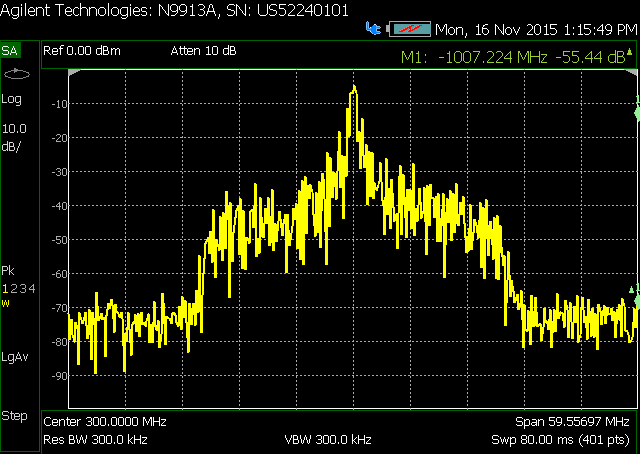
\includegraphics[scale=0.7]{NoFilter}}
		\caption{Unit Test Filtered for Matchstiq-Z1}
		\label{fig:nofilt}
	\end{figure}
	\newpage

	\begin{figure}[ht]
		\centerline{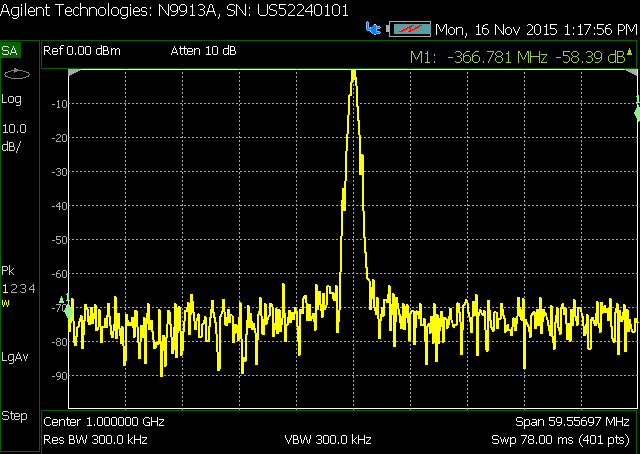
\includegraphics[scale=0.7]{YesFilter}}
		\caption{Unit Test Filtered for Matchstiq-Z1}
		\label{fig:filt}
	\end{figure}

	The signal should look like a amplitude adjusted version of the first picture throughout except when testing the filtering.  In the filtering stage of testing, the signal will slowly walk from the second picture back to the first picture.

\pagebreak
	The spectrum for the Zed/Zipper, below, is a result of the Zed/Zipper having a higher minimum sample rate of 500kHz vs 100kHz for the Matchstiq-Z1. In this case, the Zynq processor can not source sample data fast enough, which results in the output buffer underrunning. During these underrun conditions, the output of the buffer holds the last value, which results in repeated constant values being sent to the Lime transmitter.

	\begin{figure}[ht]
		\centerline{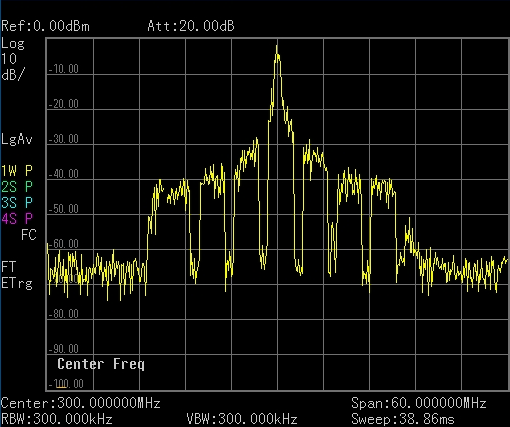
\includegraphics[scale=0.7]{NoFilter_zed_zipper}}
		\caption{Unit Test Filtered for Zed/Zipper}
		\label{fig:nofilt}
	\end{figure}
	\newpage

	\vspace{15 mm}

\end{flushleft}
\section*{References}
\begin{flushleft}
	\begin{itemize}
		\item[1)] LMS6002D Datasheet, www.limemicro.com
	\end{itemize}
\end{flushleft}
\end{document}
